\section{Le prompt du RAG} \label{appdx:prompt} 
\begin{tcolorbox}[
  colback=purple!6,        % fond pastel (modifiable)
  colframe=black,        % bord noir
  boxrule=0.8pt,         % épaisseur du cadre
  arc=0mm,               % coins légèrement arrondis
  left=6pt,
  right=6pt,
  top=6pt,
  bottom=6pt,
  fontupper=\ttfamily,   % police monospace
]
Tu es un assistant spécialisé dans les éditions numériques en humanités.\\
Réponds uniquement en te basant sur les documents fournis.\\
Cite toujours tes sources avec la date et le titre du document.
\end{tcolorbox}

\bigskip


\section{Les requêtes faites au RAG (Corpus AVH)} \label{appdx:questions_rag} 
\subsection{Cohérence des réponses lors de répétitions de questions} \label{appdx:requetesdoubles}
\paragraph{Question :} Peux-tu me citer les naissances en 1921?

\paragraph{Réponse (Version 1) :}
\begin{enumerate}
    \item Notre camarade et Mme Sibiril (Pierre), nous font part de la naissance de leur fille Suzanne, née le 2 octobre 1921.
    \item Notre camarade et Mme Colleuille (Maurice), nous font part de la naissance de leur fils Robert-Maurice, né le 8 septembre.
    \item Notre camarade et Mme Felgeirolles (Henri), nous font part de la naissance de leur fille Marie-Louise, née le 30 août.
    \item Notre camarade et Mme Fossati (André), nous font part de la naissance de leur fils Maurice, né le 27 septembre.
    \item Notre camarade et Mme Rascle (Edmond), nous font part de la naissance de leur fille Raymonde, née le 4 octobre.
    \item Notre camarade et Mme Malgoire, nous font part de la naissance de leur enfant, né le 24 septembre.
    \item Notre camarade et Mme Rouxel (E.), nous font part de la naissance de leur fille Blanche, née le 7 octobre.
    \item Notre camarade et Mme Beve (E.), nous font part de la naissance de leur fille Marthe, née le 22 octobre.
    \item Notre camarade et Mme Lamaury (Pierre), nous font part de la naissance de leur fils Fernand.
    \item Notre camarade et Mme Hassen Ben Salem Kraiem, nous font pa. de la naissance de leur fille, née le 20 octobre.
    \item Notre camarade et Mme Boucher, nous font part de la naissance de leur fils Raymond, né le 27 octobre 1921.
    \item Notre camarade et Mme Gambert (François), nous font part de la naissance de leur deuxième garçon, né le 22 septembre.
    \item Notre camarade et Mme Moteau (Jean), nous font part de la naissance de leur deuxième garçon, né le 17 octobre.
\end{enumerate}

\paragraph{Réponse (Version 2) :}
\begin{enumerate}
    \item Notre camarade et Mme Sibiril (Pierre) ont eu une fille Suzanne le 2 octobre 1921.
    \item Notre camarade et Mme Colleuille (Maurice) ont eu un fils Robert-Maurice le 8 septembre.
    \item Notre camarade et Mme Felgeirolles (Henri) ont eu une fille Marie-Louise le 30 août.
    \item Notre camarade et Mme Fossati (André) ont eu un fils Maurice le 27 septembre.
    \item Notre camarade et Mme Rascle (Edmond) ont eu une fille Raymonde le 4 octobre.
    \item Notre camarade et Mme Malgoire ont eu un enfant le 24 septembre.
    \item Notre camarade et Mme Moteau (Jean) ont eu un deuxième garçon le 17 octobre.
    \item Notre camarade et Mme Beve (E.) ont eu une fille Marthe le 22 octobre.
    \item Notre camarade et Mme Lamaury (Pierre) ont eu un fils Fernand.
    \item Notre camarade et Mme Hassen Ben Salem Kraiem ont eu une fille le 20 octobre.
    \item Notre camarade et Mme Boucher ont eu un fils Raymond le 27 octobre 1921.
    \item Notre camarade et Mme Gambert (François) ont eu leur deuxième garçon le 22 septembre.
    \item Notre camarade et Mme Rouxel (E.) ont eu une fille Blanche le 7 octobre.
    \item Notre camarade et Mme Lassalle (Auguste) ont eu une fille Augusta le 17 septembre.
    \item Notre camarade et Mme Denos (Jean) ont eu un fils Pierre le 14 octobre.
    \item Notre camarade et Mme Juif (Georges) ont eu une fille.
    \item Notre camarade et Mme Masson (François) ont eu un fils Louis le 8
\end{enumerate}

\separation

\paragraph{Question :} Qu'est-ce que la guerre ?

\paragraph{Réponse (Version 1) :}
\begin{enumerate}
\item La guerre est une action extérieure occasionnée par des événements de guerre et du fait de l'ennemi qui résulte en lésions graves et la destruction des vies humaines précieuses et des foyers (Bulletin mensuel de l'Union des aveugles de guerre et Journal des soldats blessés aux yeux - 17ème année 1935, n°2). 
\item Selon l'Union des aveugles de guerre, la guerre offensive est immorale et criminelle (Bulletin mensuel de l'Union des aveugles de guerre et Journal des soldats blessés aux yeux - 13ème année 1931, n°7). 
\end{enumerate}

\paragraph{Réponse (Version 2) :}
\begin{enumerate}
\item La guerre est l'action extérieure qui occasionne des lésions physiques à un individu pendant des événements de guerre et du fait de l'ennemi. (Source: Bulletin mensuel de l'Union des aveugles de guerre et Journal des soldats blessés aux yeux - 17ème année 1935, n°2) 
\item Quelle est la position de l'organisme sur la guerre offensive ? La guerre offensive est immorale et criminelle. (Source: Bulletin mensuel de l'Union des aveugles de guerre et Journal des soldats blessés aux yeux - 13ème année 1931, n°7)
\end{enumerate}

\subsection{Qualité des réponses à des questions diverses} \label{appdx:requetesdiverses}
\paragraph{Question :} Qu'est-ce que le vélo-car ?

\paragraph{Réponse :} The Vélocar is a bicycle that is car-like in appearance, with a structure that resembles a small automobile. It is propelled by pedaling, and it has three gears that allow it to reach speeds of up to 50 kilometers per hour and climb hills easily. The occupants pedal at their own pace, each with their own independent pedal and free wheel. (1927-12-01, Bulletin mensuel de l'Union des aveugles de guerre et Journal des soldats blessés aux yeux - 9ème année 1927 n°10)

\separation

\paragraph{Question :} Qu'est-ce qu'un aveugle de guerre ?

\paragraph{Réponse :}
According to the "Bulletin mensuel de l'Union des aveugles de guerre et Journal des soldats blessés aux yeux - 5ème année 1923, n°3" on 1923-03-01, an aveugle de guerre is not an invalid, but a mutilé; the difference is great. He is a man who, by virtue of a worldwide catastrophe, has lost the use of one of his senses, but who has not lost his intelligence, activity, skill, and the memory of everything he has seen. He can compensate for the sudden loss of his sight through new tactile and auditory"

\separation

\paragraph{Question :} La vie ...

\paragraph{Réponse :}
The life of the blind veterans is discussed in the documents, particularly their pensions, rehabilitation, employment, and social aide. For example, in the document "Bulletin mensuel de l'Union des aveugles de guerre et Journal des soldats blessés aux yeux - 5ème année 1923, n°1", there is a questionnaire about Franceville, a home for the blind veterans ...

\subsection{Neutralité pour des questions non pertinentes} \label{appdx:requetesnonpertinentes}
\paragraph{Question :} Qui a volé l'orange du marchand ?

\paragraph{Réponse :} The document does not provide information about someone stealing an orange from a merchant.

\separation

\paragraph{Question :} Qu'est-ce que l'iphone ?

\paragraph{Réponse :} L'iphone n'est pas mentionné dans les documents fournis, il est impossible de répondre à la question avec précision en se basant sur les documents.

\section{Détails des retours de requêtes (Corpus AVH)} \label{appdx:details_rag}
\begin{figure}[h!]
  \centering
  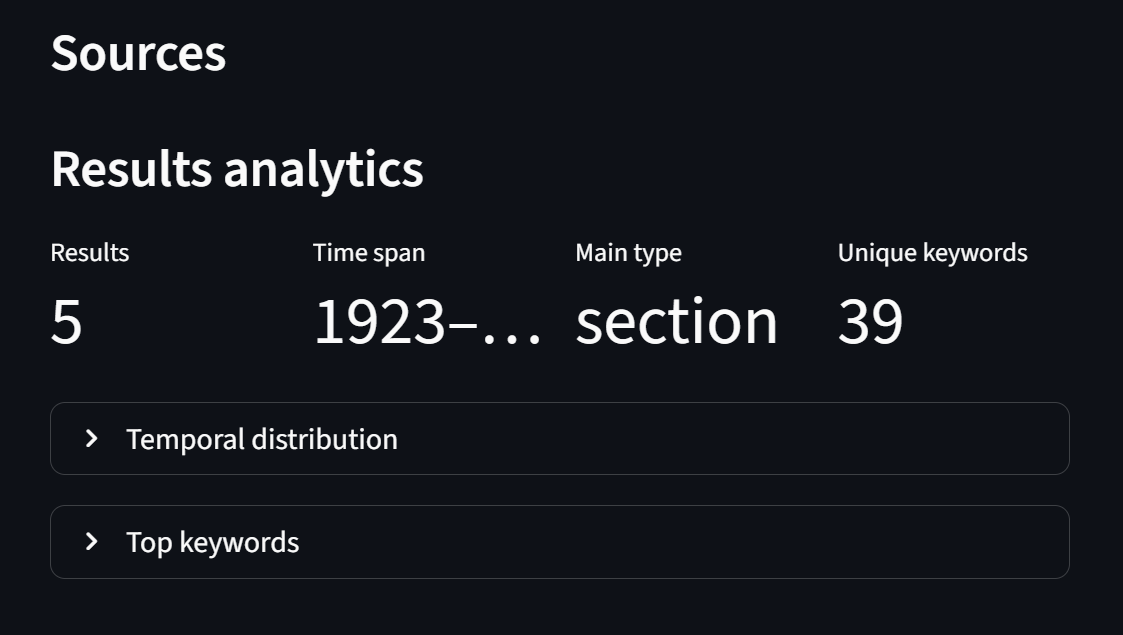
\includegraphics[width=0.8\linewidth]{images/analytics_1.png}
  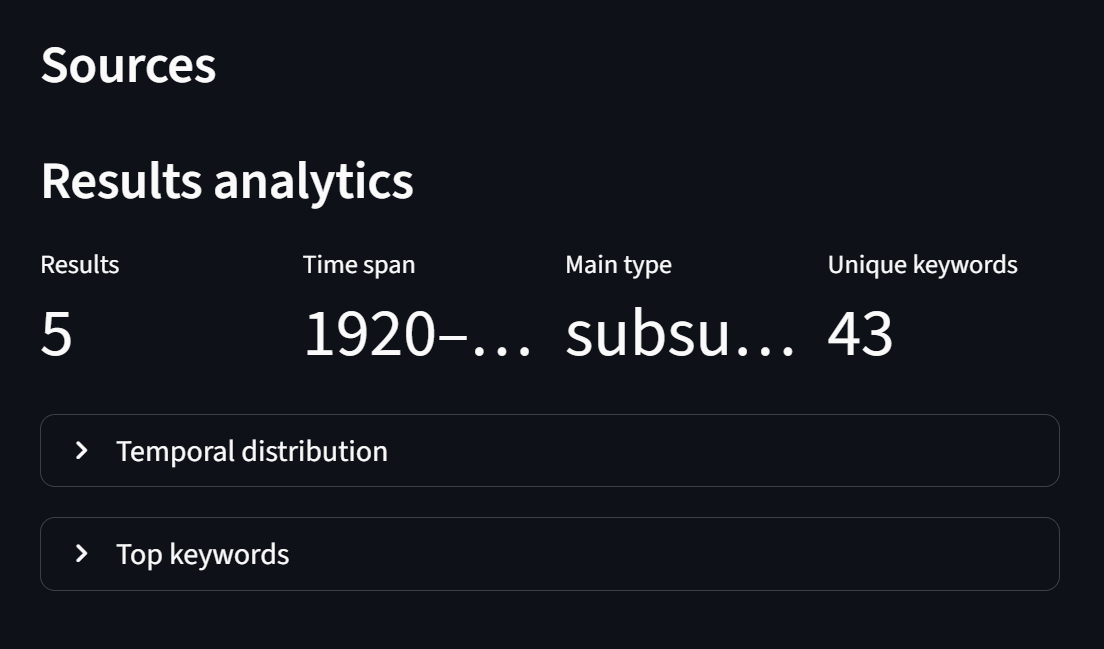
\includegraphics[width=0.8\linewidth]{images/analytics_2.png}
  \caption{Retour général après requête}
  \label{appdx:retourgeneral}
\end{figure}

\begin{figure}[p!]
  \centering
  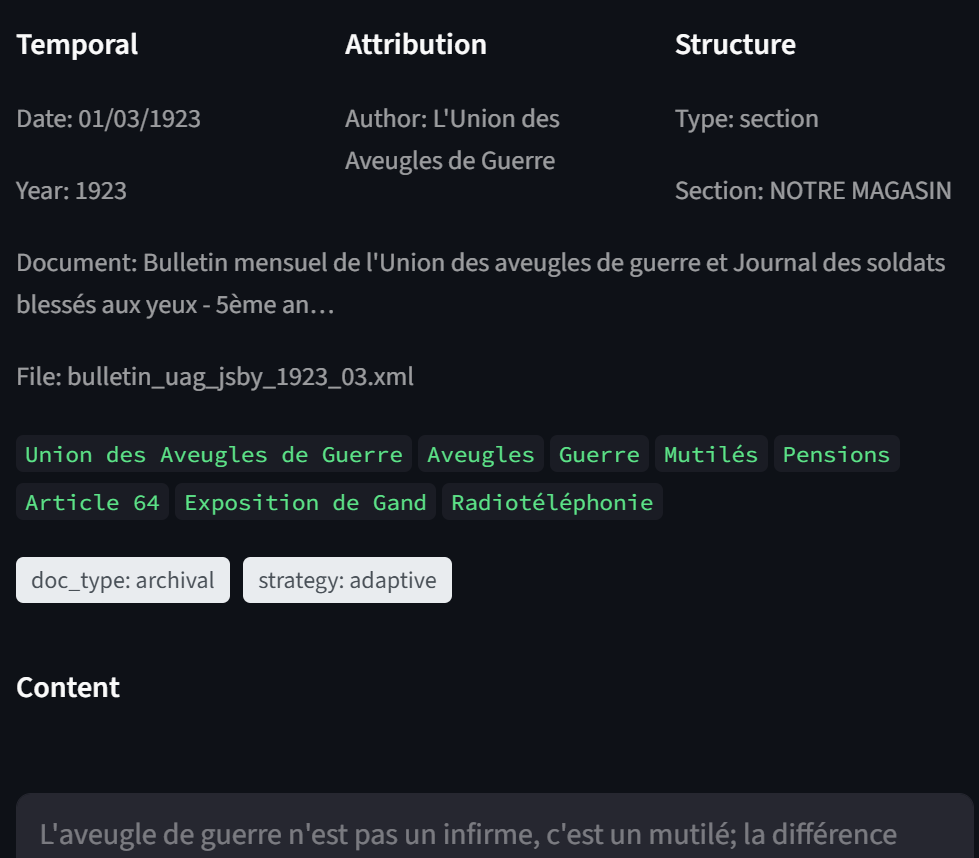
\includegraphics[width=0.6\linewidth]{images/details_1.png}
  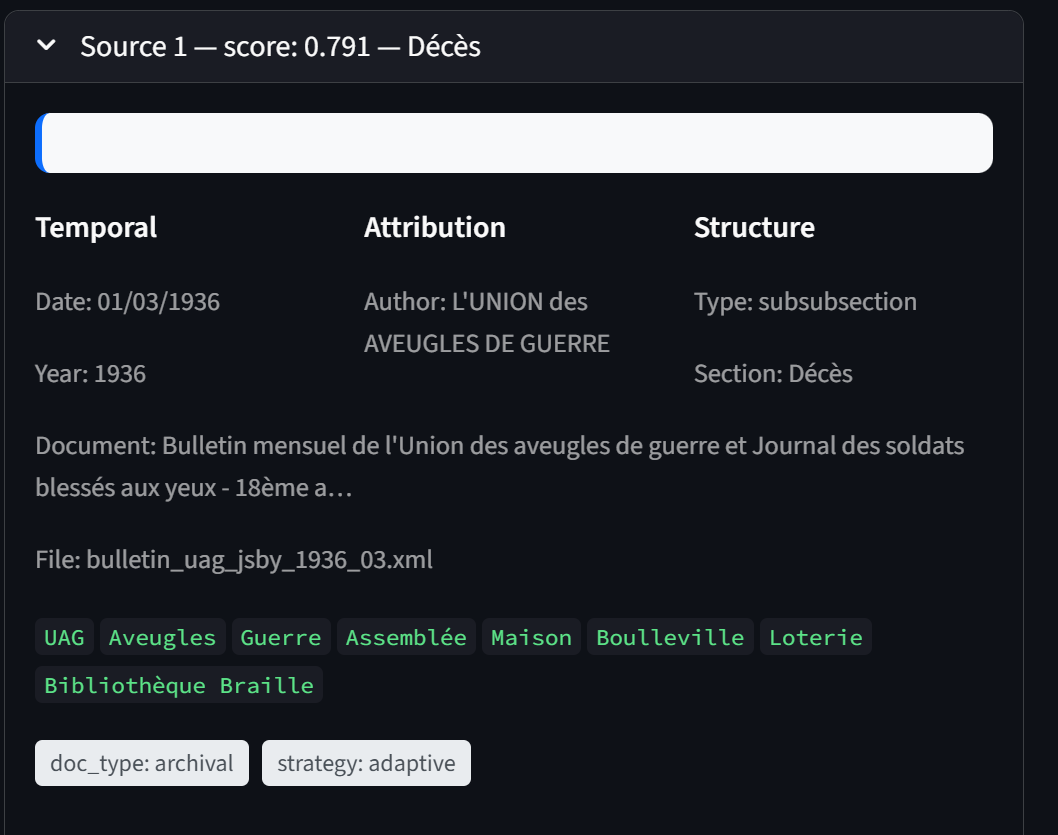
\includegraphics[width=0.6\linewidth]{images/details_2.png}
  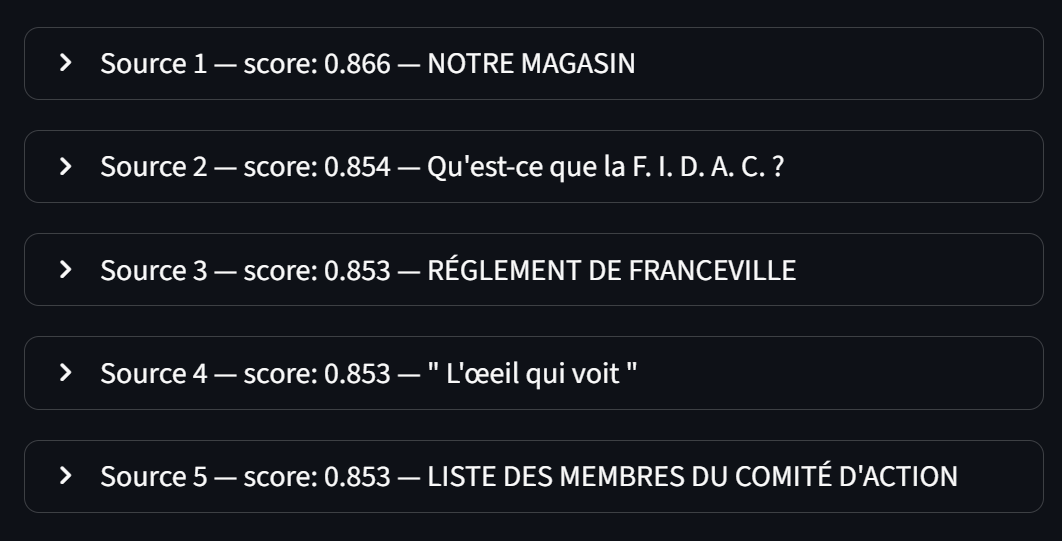
\includegraphics[width=0.6\linewidth]{images/details_3.png}
  \caption{Retour par source après requête}
  \label{appdx:retourparsource}
\end{figure}

\newpage
\section{Les requêtes faites au RAG (Corpus Paul d'Estournelles)} \label{appdx:questions_rag_pec} 
\bigskip
\paragraph{Question : } Comment s'appelle la fille de Paul d'Estournelles

\paragraph{Réponse}
The daughter of Paul d'Estournelles is named Henriette. \\ Reference(s): - doc\_title: Letter number 850 from Paul d'Estournelles de Constant to Nicholas Murray Butler (June 23, 1921) - file\_name: Lettre0850\_23juin1921.xml

\separation

\paragraph{Question : } Les Italiens

\paragraph{Réponse : }
\begin{enumerate}
    \item Les Italiens ont été irrités contre les Français, les Anglais et les Américains (Letter number 724 from Paul d'Estournelles de Constant to Nicholas Murray Butler, November 26, 1920).
    \item Les Italiens ont reçu une acclamation pour le fascisme, qui réclame la Dalmatie, l'Adriatique, la Méditerranée, Nice, la Savoie, la Corse, la Tunisie, une partie de la Suisse, etc., et a tendu la main au féodalisme Hongrois contre les Slaves des Balkans (Letter number 1206 from Paul d'Estournelles de Constant to Nicholas Murray Butler, November 29, 1922).
    \item Les Italiens ne disent rien ni de Trieste, ni du Trentin, mais pensent aux sacrifices dont ils faut payer pour aboutir à des succès actuels. Ils ont également souligné que si les Allemands envahissent de nouveau la Péninsule, il n'est pas clair de savoir si il est la peine de se ruiner pour aboutir à ce résultat (Letter number 713 from Paul d'Estournelles de Constant to Nicholas Murray Butler, October 19, 1920).
\end{enumerate}

\separation

\paragraph{Question : } Qui est Elihu Root ?

\paragraph{Réponse : } Elihu Root is a person who is mentioned in the letters from Paul d'Estournelles de Constant to Nicholas Murray Butler, specifically in the documents "Letter number 1451 from Paul d'Estournelles de Constant to Nicholas Murray Butler (December 4, 1923)" and "Letter number 1438 from Paul d'Estournelles de Constant to Nicholas Murray Butler (November 22, 1923)". \\ 
Elihu Root was a prominent American statesman, lawyer, and academic who served as the United States Secretary of War and Secretary of State. He was also the President of the Carnegie Endowment for International Peace. \\
Reference(s): - "Letter number 1451 from Paul d'Estournelles de Constant to Nicholas Murray Butler (December 4, 1923)", 1957 - "Letter number 1438 from Paul d'Estournelles de Constant to Nicholas Murray Butler (November 22, 1923)", 1957

\separation

\paragraph{Question}
Prix Nobel de la Paix

\paragraph{Réponse}
Based on the provided documents, the Nobel Peace Prize is not directly mentioned. However, in letter number 407 from Paul d'Estournelles de Constant to Nicholas Murray Butler dated August 9, 1918, it is mentioned that the Carnegie Endowment for International Peace is offering its services to the U.S. government to help treat international affairs related to the war. This organization was established by Andrew Carnegie, who received the Nobel Peace Prize in 1911. (1957, 1957)

\separation

\paragraph{Question : } Traité de Versailles

\paragraph{Réponse : }
\begin{enumerate}
    \item The Treaty of Peace has been proclaimed and it will have to become a reality. (Letter number 14 from Paul d'Estournelles de Constant to Nicholas Murray Butler, December 3, 1914)
    \item The Treaty of Versailles has been signed, but it remains to be applied and amended in such a way that this war truly ends and cannot resume. (Letter number 622 from Paul d'Estournelles de Constant to Nicholas Murray Butler, February 15, 1920)
    \item The Treaty of Peace, as it was proclaimed in a letter from Paul d'Estournelles de Constant to Nicholas Murray Butler on December 3, 1914 \\ (ref. Lettre0014\_3decembre1914.xml).
    \item The Treaty of Versailles, which was signed but not yet executed, according to a statement in a letter from Paul d'Estournelles de Constant to Nicholas Murray Butler on September 18, 1923 (ref. Lettre1391\_18septembre1923.xml).
    \item The Treaty of Versailles, which Germany has signed but is yet to be applied and amended to ensure the cessation of the war in a letter from Paul d'Estournelles de Constant to Nicholas Murray Butler on February 15, 1920 (ref. Lettre0622\_15fevrier1920.xml).
    \item The Treaty of Versailles, which Germany has accepted without conditions in a letter from Paul d'Estournelles de Constant to Nicholas Murray Butler on June 24, 1919 (ref. Lettre0552\_24juin1919.xml).
\end{enumerate}

\bigskip 

\section{Les requêtes faites au RAG (Corpus EHRI)} \label{appdx:questions_rag_ehri} 
\bigskip
\paragraph{Question : } La déportation des Juifs vers Auschwitz

\paragraph{Réponse : } Les textes fournis décrivent des déportations de Juifs vers Auschwitz-Birkenau. Les témoignages de Otto Kalwo et Eduard de Wind font mention de cette destination. (Documents EHRI-DC-054\_DE\_EN.xml et EHRI-DC-066\_DE\_EN.xml)

\separation

\paragraph{Question : } Comment est la vie dans le ghetto de terezin ?

\paragraph{Réponse : } La vie dans le ghetto de Terezin était difficile. Les barracks étaient surpeuplés, une grande partie des ghettoisés devaient dormir sur le sol, car tout espace était utilisé comme lieu de sommeil. Sans lits, sans matelas ou sacs à paillasses, seulement quelques-uns étaient temporairement disponibles. Les campagnards dormaient sur des sols froids, beaucoup d'entre eux dans des salles telles que les écuries, les entrepôts et les lieux similaires sur le sol de ciment dur. Dans les baraques des Sudè

\separation

\paragraph{Question : } attaque antisémite violente

\paragraph{Réponse : } The documents provide multiple evidence of violent anti-Semitic attacks in Slovakia. In the memorandum by the Association of the Victims of Racial Persecution Košice chapter, they mention anti-Jewish riots (doc\_title: Memorandum on anti-Jewish riots in Slovakia, Memorandum zu antijüdischen Ausschreitungen in der Slowakei, Memorandum o protižidovských nepokojích na Slovensku, paragraph xml\_id: ). Furthermore, the Association of the Victims of Racial Persecution, eastern district of Košice, ...

\separation

\paragraph{Question : } hitler

\paragraph{Réponse : } The query "hitler" does not appear in the provided documents.

\separation

\paragraph{Question}
Aggression non juive

\paragraph{Réponse}
At the personal level, the persecution is even more severe. Association with Germans is strictly forbidden, and even kids are not allowed to play with German kids. Although in legal terms we are not expelled from the country, the method used goes against humanity and arouses (uncontrollable) anger. (Giuseppe Talamo Atenolfi on Hungarian actions against Jews in occupied Galicia in 1942, Giuseppe Talamo Atenolfi über ungarische Aktionen gegen Juden im besetzten Galizien im Jahr 1942, EHRI-DR-19

\separation

\paragraph{Question : } Aggression non-juive

\paragraph{Réponse : }
\begin{enumerate}
    \item In the document "A fifteen-year-old youth, on the German invasion of Wyszków and surrounding areas" written on an undetermined date, the author describes how Jews were severely beaten. (keywords: testimony, robberies, beaten) 
    \item In the document "Ray Atherton on the reaction of the non-Jewish Bulgarian population towards antisemitic demonstrations in 1939", the author mentions that there is no sympathy in Bulgaria for the antisemitic demonstrations of the organization "Workers of New Bulgaria" ...
\end{enumerate}

\separation

\paragraph{Question : } Qui est persecuté outre les juifs

\paragraph{Réponse : } Les juifs sont persecutés en plus de quelqu'un d'autre, mais il n'est pas spécifié dans les documents fournis qui sont les autres personnes qui sont persecutées.